%-----------------------Homework------------------------------------
%-------------------Arman Shokrollahi---------------------------------
%---------------------Introduction to Electrical and Electronic Engineering-------------------------------

\documentclass[a4 paper]{article}
% Set target color model to RGB
\usepackage[inner=1.5cm,outer=1.5cm,top=2.5cm,bottom=2.5cm]{geometry}
\usepackage{setspace}
\usepackage[rgb]{xcolor}
\usepackage{verbatim}
\usepackage{amsgen,amsmath,amstext,amsbsy,amsopn,tikz,amssymb,tkz-linknodes}
\usepackage{fancyhdr}
\usepackage[colorlinks=true, urlcolor=blue,  linkcolor=blue, citecolor=blue]{hyperref}
\usepackage[colorinlistoftodos]{todonotes}
\usepackage{rotating}
\usepackage{multirow}
\usepackage{graphicx}
\usepackage{paracol}
\usepackage{color}
\newcommand{\blue}[1]{\textcolor{blue}{#1}}
\newcommand{\red}[1]{\textcolor{red}{#1}}
\newcommand{\green}[1]{\textcolor{green}{#1}}
\newcommand{\yellow}[1]{\textcolor{yellow}{#1}}
\newcommand{\orange}[1]{\textcolor{orange}{#1}}
\newcommand{\violet}[1]{\textcolor{violet}{#1}}

%\usetikzlibrary{through,backgrounds}
\hypersetup{%
pdfauthor={Nan Meng},%
pdftitle={Notes},%
pdfkeywords={Tikz,latex,bootstrap,uncertaintes},%
pdfcreator={PDFLaTeX},%
pdfproducer={PDFLaTeX},%
}
%\usetikzlibrary{shadows}
\usepackage[francais]{babel}
\usepackage{booktabs}
\newcommand{\ra}[1]{\renewcommand{\arraystretch}{#1}}

      \newtheorem{thm}{Theorem}[section]
      \newtheorem{prop}[thm]{Proposition}
      \newtheorem{lem}[thm]{Lemma}
      \newtheorem{cor}[thm]{Corollary}
      \newtheorem{defn}[thm]{Definition}
      \newtheorem{rem}[thm]{Remark}
      \numberwithin{equation}{section}

\newcommand{\homework}[6]{
   \pagestyle{myheadings}
   \thispagestyle{plain}
   \newpage
   \setcounter{page}{1}
   \noindent
   \begin{center}
   \framebox{
      \vbox{\vspace{2mm}
    \hbox to 6.28in { {\bf ENGG1203:~Introduction to Electrical and Electronic Engineering \hfill} }
       \vspace{6mm}
       \hbox to 6.28in { {\Large \hfill #1 (#2)  \hfill} }
       \vspace{6mm}
       \hbox to 6.28in { {\it Instructor: #3 \hfill TA: #5} }
       %\hbox to 6.28in { {\it TA: #4  \hfill #6}}
      \vspace{2mm}}
   }
   \end{center}
   \markboth{#5 -- #1}{#5 -- #1}
   \vspace*{4mm}
}

\newcommand{\bbF}{\mathbb{F}}
\newcommand{\bbX}{\mathbb{X}}
\newcommand{\bI}{\mathbf{I}}
\newcommand{\bX}{\mathbf{X}}
\newcommand{\bY}{\mathbf{Y}}
\newcommand{\bepsilon}{\boldsymbol{\epsilon}}
\newcommand{\balpha}{\boldsymbol{\alpha}}
\newcommand{\bbeta}{\boldsymbol{\beta}}
\newcommand{\0}{\mathbf{0}}

\begin{document}
\homework{\bf Circuits}{ENGG1203}{Edmund Y.Lam}{}{Nan Meng}{}

% {\begin{tikzpicture}[outline/.style={draw=#1,thick,fill=#1!50}]
% \node [outline=red] at (0,1) {\bf Problem 1};
% \end{tikzpicture}}

\section{Operational Amplifier}
An operational amplifier(op-amp) is a voltage controlled voltage source with high gain. The equivalent circuit model of an op-amp is shown on Figure \ref{op-amp}. The voltage $V_i$ is the differential input voltage $V_i = V_p - V_n$.  $R_i$ is the input resistance of the device and $R_o$ is the output resistance. The gain parameter $A$ is called the open loop gain.
\begin{figure}[!ht]
  \centering
  \label{op-amp}
  \includegraphics[width=0.4\textwidth]{./images/circuit2/circuit_append}
  \caption{{\bf Equivalent circuit model of op-amp device}}
\end{figure}

If there is no load at the output, the output voltage is 
\begin{equation}
V_o = AV_i = A(V_p-V_n)
\end{equation}

From the equation above, output voltage $V_o$ is a function of the difference between the input voltage $V_p$ and $V_n$. For this reason, the op-amps are also called {\bf difference amplifiers}.

The figure that reflects relation between the output voltage and the input voltage is called the voltage transfer curve and is fundamental in designing and understanding amplifier circuits. The voltage transfer curve of the op-amp is shown on Figure 2.%\ref{op-amp_curve}. 

\begin{figure}[!ht]
  \centering
  \label{op-amp_curve}
  \includegraphics[width=0.4\textwidth]{./images/op_amp_curve}
  \caption{{\bf Op-amp voltage transfer characteristics}}
\end{figure}




\subsection{The ideal op-amp model}
Practically speaking, an ideal op-amp is a device which acts as an ideal voltage controlled voltage source. Referring to Figure 3, this implies that the device will have the following characteristics: 

\begin{itemize}
  \item[$\ast$] No current flows into the input terminals of the device. This is equivalent to having an infinite input resistance $R_i = \infty$. In practical terms this implies that the amplifier device will make no power demands on the input signal source.
  \item[$\ast$] Have a zero output resistance$(R_o = 0)$. This implies that the output voltage is independent of the load connected to the output.
\end{itemize}



In addition the ideal op-amp model will have infinite open loop gain$(A \rightarrow \infty)$. The ideal op-amp model can be shown schematically on Figure 3.%\ref{op-amp2}.


\begin{figure}[!ht]
  \centering
  \label{op-amp2}
  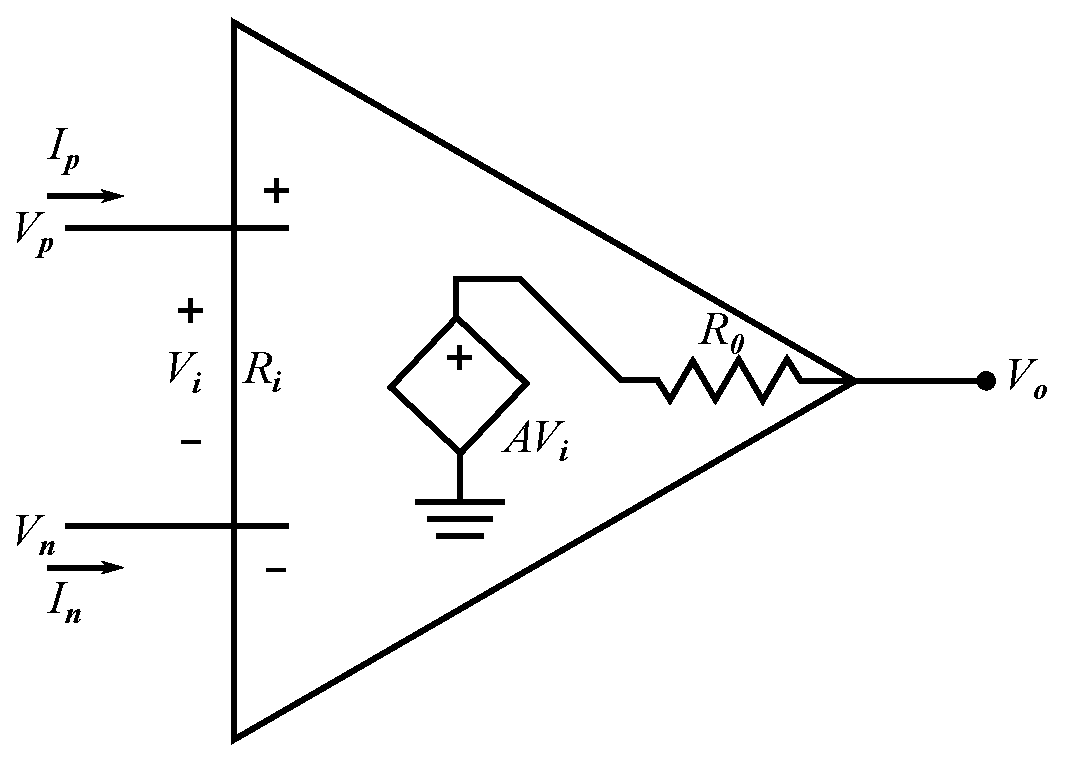
\includegraphics[width=0.4\textwidth]{./images/circuit2/circuit_append1}
  \caption{{\bf Op-amp voltage transfer characteristics}}
\end{figure}

In summary, the ideal op-amp conditions are: 

\begin{itemize} \itemsep3pt \parskip0pt \parsep0pt
  \item[$\bullet$] $I_p = I_n = 0$ \hspace{8 mm}\blue{\bf No current into the input terminals}
  \item[$\bullet$] $I_p = I_n = 0$ \hspace{8 mm}\blue{\bf No current into the input terminals}
  \item[$\bullet$] $R_i = \infty$ \hspace{14 mm}\blue{\bf Infinite input resistance}
  \item[$\bullet$] $R_0 = 0$ \hspace{15 mm}\blue{\bf Zero output resistance}
\end{itemize}

Even though real op-amps deviate from these ideal conditions, the ideal op-amp rules are very useful and are used extensively in circuit design and analysis.


\subsection{Ideal op-amp in a negative feedback configuration}


When an op-amp is arranged with a negative feedback the ideal rules are:

\begin{itemize} \itemsep3pt \parskip0pt \parsep0pt
  \item[$\bullet$] $I_p = I_n = 0$ \hspace{8 mm} \blue{\bf input current constraint}
  \item[$\bullet$] $V_n = V_p$ \hspace{13.5 mm} \blue{\bf input voltage constraint}
\end{itemize}


\begin{figure}[!ht]
  \centering
  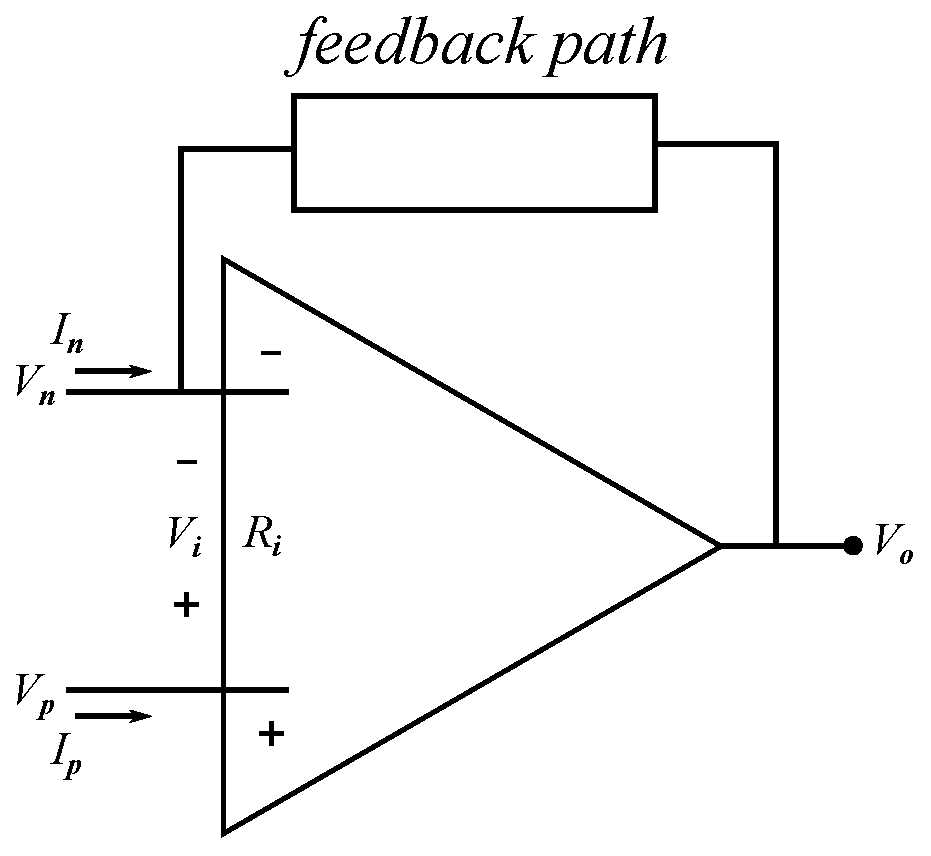
\includegraphics[width=0.3\textwidth]{./images/circuit2/circuit_append2}
  \caption{{\bf Op-amp voltage transfer characteristics}}
\end{figure}

\subsection{Computational Devices}

So far we have explored the use of op amps to multiply a signal by a constant. For the inverting amplifier the multiplication constant is the gain $-\frac{R_2}{R_1}$ and for the non inverting amplifier the multiplication constant is the gain $1 + \frac{R_2}{R_1}$. Op amps may also perform other mathematical operations ranging from addition and subtraction to integration, differentiation and exponentiation. We will next explore these fundamental ``operational'' circuits.

\subsubsection{Summing Amplifier}
A basic summing amplifier circuit with three input signals is shown in Figure 5.


\begin{figure}[!ht]
  \centering
  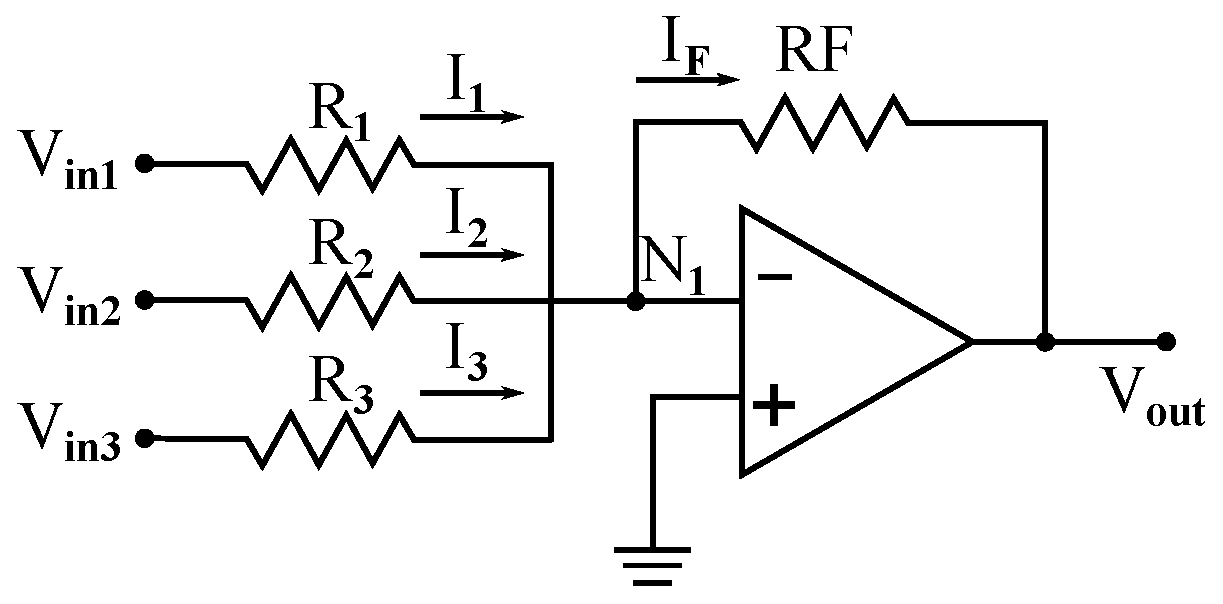
\includegraphics[width=0.5\textwidth]{./images/summingamp}
  \caption{{\bf Summing Amplifier}}
\end{figure}

Apply KCL at Node {\bf N1}:

\begin{equation}
I_1 + I_2 + I_3 = I_F
\end{equation}

By relating the currents $I_1$, $I_2$ and $I_3$ to their corresponding voltage and resistance by Ohm's law:

\begin{equation}
\frac{V_{in1}}{R_1} + \frac{V_{in2}}{R_2} + \frac{V_{in3}}{R_3} = -\frac{V_{out}}{RF}
\end{equation}

So $V_{out}$ is:

\begin{equation}
V_{out} = -(\frac{RF}{R_1}V_{in1}+\frac{RF}{R_2}V_{in2}+\frac{RF}{R_3}V_{in3})
\end{equation}
From the expression (1.4), $V_{out}$ is a sum of the input voltages with weighting factors given by the values of the resistors. If $R_1 = R_2 = R_3 = R$, then we will get:

\begin{equation}
V_{out} = -\frac{RF}{R}(V_{in1} + V_{in2} + V_{in3})
\end{equation}

The output voltage is the sum of the input voltages with a multiplication constant \blue{$\frac{RF}{R}$}. For a special case when $RF = R$, the output voltage is the sum of the inputs:

\begin{equation}
V_{out} = -(V_{in1} + V_{in2} + V_{in3})
\end{equation}


The input resistance seen by each source connected to the summing amplifier is the corresponding series resistance connected to the source. Therefore, the sources do not interact with each other.


\subsubsection{Difference Amplifier}
This fundamental op amp circuit, shown on Figure 2, amplifies the difference between the input signals. The subtracting feature is evident from the circuit configuration which shows that one input signal is applied to the inverting terminal and the other to the non-inverting terminal.

\begin{figure}[!ht]
  \centering
  \includegraphics[width=0.5\textwidth]{./images/differenceamp}
  \caption{{\bf Difference Amplifier}}
\end{figure}

\begin{equation}
V_- = \frac{V_{out}-V_{in1}}{R_1+R_2}R_1 + V_{in1} = \frac{R_1}{R_1 + R_2}V_{out} + \frac{R_2}{R_1 + R_2}V_{in1}
\end{equation}
\begin{equation}
V_+ = \frac{R_4}{R_3 + R_4}V_{in2}
\end{equation}

From the input voltage constraint($V_+ = V_-$), the output voltage is:
\begin{equation}
V_{out} = V_{in2}(\frac{R_4}{R_3+R_4})(1+\frac{R_2}{R_1})-V_{in1}\frac{R_2}{R_1}
\end{equation}

Note that in order to have a subtracting circuit which gives V out =0 for equal inputs, the weight of each signal must be the same. Therefore

\begin{equation}
(\frac{R_4}{R_3 + R_4})(1 + \frac{R_2}{R_1}) = \frac{R_2}{R_1}
\end{equation}
which holds only if
\begin{equation}
\frac{R_4}{R_3} = \frac{R_2}{R_1}
\end{equation}
The output voltage is now
\begin{equation}
V_{out} = \frac{R_2}{R_1}(V_{in2} - V_{in1})
\end{equation}

which is a difference amplifier with a differential gain of $R_2/R_1$ and with zero gain for the common mode signal. It is often practical to select resistors such as $R_4=R_2$ and $R_3=R_1$.


\subsubsection{Buffer Amplifier}
A {\bf buffer amplifier} (sometimes simply called a buffer) is one that provides electrical impedance transformation from one circuit to another. A buffer is something that isolates or separates one circuit from another. 

\begin{figure}[!ht]
  \centering
  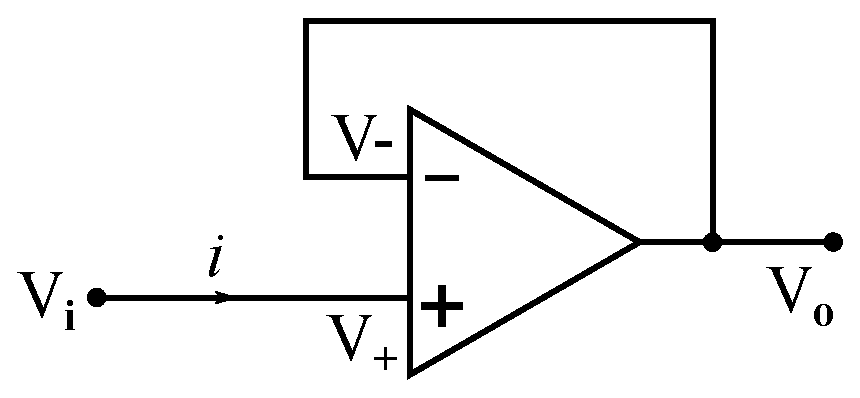
\includegraphics[width=0.3\textwidth]{./images/buffer}
  \caption{{\bf Buffer Amplifier}}
\end{figure}

\begin{equation}
i = 0
\end{equation}
\begin{equation}
v_o = v_i(=v_-=v_+)
\end{equation}

A {\bf buffer} is a {\bf unity-gain} amplifier that has an extremely high input resistance and an extremely low output resistance. This means that the buffer can be modeled as a voltage controlled voltage source that has a gain of one.


\subsubsection{Non-inverting\&inverting Amplifier}



\begin{paracol}{2}
\begin{leftcolumn*}

\begin{figure}[ht]
  % \caption{Non-inverting Amplifier}
  \label{Non-inverting Amplifier}
  \centering
  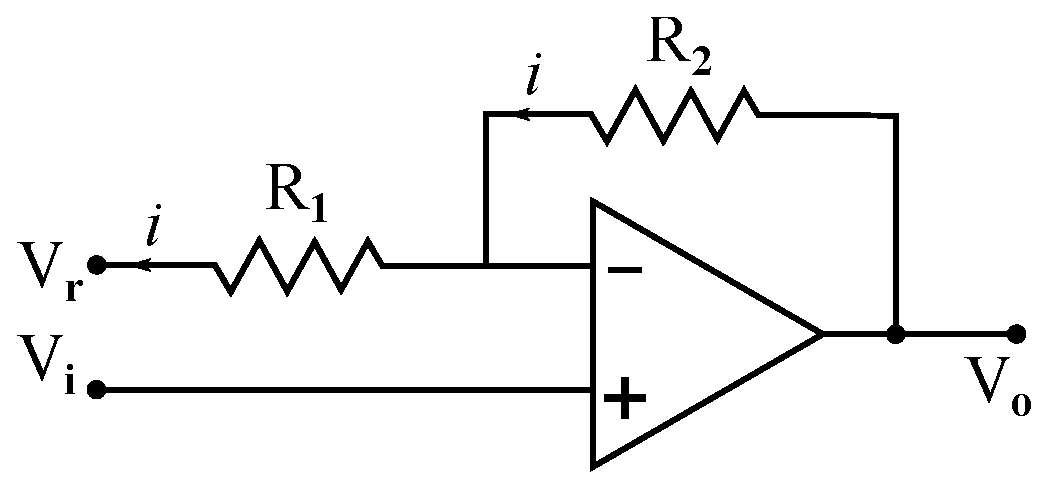
\includegraphics[width=0.3\textwidth]{./images/non-inverting}
\end{figure}

Amplify difference with reference voltage
\begin{equation}
v_o-v_r = (1+\frac{R_2}{R_1})(v_i-v_r)
\end{equation}


\end{leftcolumn*}

\begin{rightcolumn}

\begin{figure}[ht]
  % \caption{Inverting Amplifier}
  \label{Inverting Amplifier}
  \centering
  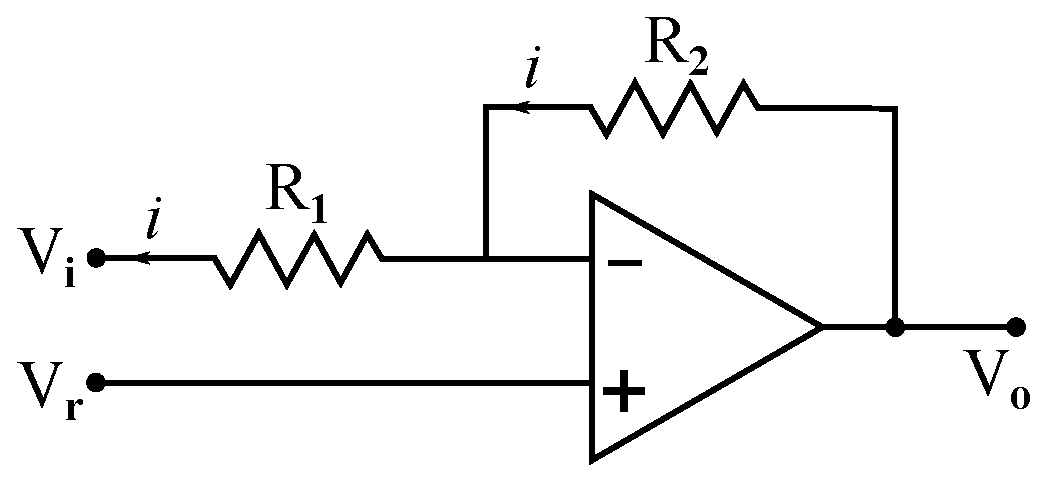
\includegraphics[width=0.3\textwidth]{./images/inverting}
\end{figure}
{Amplify and invert difference with reference voltage}
\begin{equation}
v_o-v_r = -\frac{R_2}{R_1}(v_i-v_r)
\end{equation}

\end{rightcolumn}
\end{paracol}














%
%
\end{document}
%%------------------ Arman Shokrollahi--------------%%
